% !TeX spellcheck = de_DE
\documentclass{uebung_cs}
\usepackage{algo121}
\blattname{\emoji{star}-Aufgabe: Flaschenhals}

%%%%%%%%%%%%%%%%%%%%%%%%%%%%%%%%%%%%%%%%%%%%%%%%%%%%%%%%%%%%%%%%%%%%%%%%%%%%
\begin{document}
\textit{\footnotesize For an English version of this exercise, see [\href{https://jeffe.cs.illinois.edu/teaching/algorithms/book/Algorithms-JeffE.pdf}{Erickson}, page 270]}.

  Betrachte einen einfachen Weg zwischen zwei Knoten $s$ und $t$ in einem ungerichteten, gewichteten Graphen $G$.
  Die \emph{Breite} dieses Wegs ist das minimale Gewicht, das auf den Kanten des Wegs vorkommt.
  Die Flaschenhals-Distanz zwischen $s$ und $t$ ist die Breite des breitesten einfachen Wegs von $s$ nach $t$. (Wenn es keinen Weg von $s$ nach $t$ gibt, ist die Flaschenhals-Distanz $-\infty$. Die Flaschenhals-Distanz von $s$ nach $s$ ist $\infty$.)
  \begin{center}
    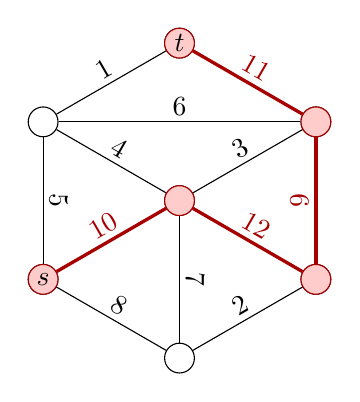
\begin{tikzpicture}[minimum size=2.5ex,inner sep=0,
        emphedge/.style={very thick,color=red!65!black},
        emphnode/.style={draw=red!65!black,circle,fill=red!20!white},
        ]
        \foreach \i in {0,...,5}{
            \node[draw,circle] (v\i) at (\i*360/6+90:2) {};
        }
        \node[draw,circle] (c) at (0,0) {};

        \node[emphnode] at (v0) {$t$};
        \node[emphnode] at (v2) {$s$};
        \node[emphnode] at (c) {};
        \node[emphnode] at (v4) {};
        \node[emphnode] at (v5) {};

        \path (c) edge node[auto,sloped] {$4$} (v1)
                  edge[emphedge] node[auto,sloped] {$10$} (v2)
                  edge node[auto,sloped] {$7$} (v3)
                  edge[emphedge] node[auto,sloped] {$12$} (v4)
                  edge node[auto,sloped] {$3$} (v5);
        \path (v1) edge node[auto,sloped] {$6$} (v5);
        \path (v0) edge node[auto,sloped] {$1$} (v1);
        \path (v1) edge node[auto,sloped] {$5$} (v2);
        \path (v2) edge node[auto,sloped] {$8$} (v3);
        \path (v3) edge node[auto,sloped] {$2$} (v4);
        \path (v4) edge[emphedge] node[auto,sloped] {$9$} (v5);
        \path (v5) edge[emphedge] node[auto,sloped] {$11$} (v0);
        \end{tikzpicture}

        \small Die Flaschenhals-Distanz von $s$ nach $t$ ist $9$.
  \end{center}
  \begin{enumerate}
      \item Beweise, dass der \emph{maximale} Spannbaum von $G$ zwischen \emph{jedem} Paar von Knoten einen breitesten Weg enthält.
      \item Entwirf einen Algorithmus, der das folgende Problem in $O(n+m)$ Zeit löst:
      Gegeben ein ungerichteter, gewichteter Graph~$G$ mit zwei Knoten $s$ und $t$ sowie einem Gewicht~$W$, ist die Flaschenhals-Distanz von $s$ nach $t$ höchstens $W$?
      \item Sei $B$ die Flaschenhals-Distanz von $s$ nach $t$.
        \begin{enumerate}[label=\roman*.]
            \item Beweise, dass sich die Flaschenhals-Distanz von $s$ nach $t$ nicht ändert, wenn man eine beliebige Kante von Gewicht kleiner $B$ löscht.
            \item Beweise, dass sich die Flaschenhals-Distanz von $s$ nach $t$ nicht ändert, wenn man eine beliebige Kante von Gewicht größer $B$ \emph{kontrahiert}.
            (Um eine Kante $e=\{u,v\}$ in $G$ zu kontrahieren, wird die Kante $e$ gelöscht und die beiden Endpunkte $u$ und $v$ werden zu einem neuen Knoten $w$ verschmolzen. Falls dabei parallele Kanten entstehen, behalten wir nur die 
            \emph{schwerste} Kante zwischen jedem Paar von Knoten, und löschen die anderen. Der neue Graph heißt $G/e$.)
        \end{enumerate}
    \item(\veryhard)
    Entwirf einen Algorithmus, der in Zeit $O(n+m)$ einen breitesten Weg von~$s$ nach~$t$ berechnet.
    \emph{Hinweis: Du darfst hierfür annehmen, dass man den Median von $m$ Zahlen in Zeit $O(m)$ berechnen kann.}
  \end{enumerate}
  
  \paragraph*{Hinweise zur Abgabe.}
  In den Aufgabenteilen a und c werden mathematische Beweise erwartet, und in den Aufgabenteilen b und d die übliche Struktur (grobe Idee, Pseudocode, Korrektheitsbeweis, Laufzeitanalyse).
  Um einen \emoji{star} zu erhalten, müssen die Aufgabenteile a, b und c vollständig bearbeitet werden.
\end{document}
